\documentclass[twoside,11pt]{article}

\usepackage[preprint]{jmlr2e}
\usepackage{amsmath}
\allowdisplaybreaks
\usepackage{pdfpages}


\title{02450 Report 1}
\author{{Gisle Joe Garen (s242712)} \and {Ignacio Ripoll González (s242875)} \and {Sebastian Svelmøe Timm (s243935)}}
\date{\today}

%%%%%%%%%%%%%%%%%%%%%%%%%%
%% DO NOT TOUCH
%%%%%%%%%%%%%%%%%%%%%%%%%%
    \usepackage[breakable]{tcolorbox}

    % Basic figure setup, for now with no caption control since it's done
    % automatically by Pandoc (which extracts ![](path) syntax from Markdown).
    \usepackage{graphicx}
    % Keep aspect ratio if custom image width or height is specified
    \setkeys{Gin}{keepaspectratio}
    % Maintain compatibility with old templates. Remove in nbconvert 6.0
    \let\Oldincludegraphics\includegraphics
    % Ensure that by default, figures have no caption (until we provide a
    % proper Figure object with a Caption API and a way to capture that
    % in the conversion process - todo).
    \usepackage{caption}
    % \DeclareCaptionFormat{nocaption}{}
    % \captionsetup{format=nocaption,aboveskip=0pt,belowskip=0pt}

    \usepackage{float}
    \floatplacement{figure}{H} % forces figures to be placed at the correct location
    \usepackage{xcolor} % Allow colors to be defined
    \usepackage{enumerate} % Needed for markdown enumerations to work
    \usepackage{geometry} % Used to adjust the document margins
    \usepackage{amsmath} % Equations
    \usepackage{amssymb} % Equations
    \usepackage{textcomp} % defines textquotesingle
    % Hack from http://tex.stackexchange.com/a/47451/13684:
    \AtBeginDocument{%
        \def\PYZsq{\textquotesingle}% Upright quotes in Pygmentized code
    }
    \usepackage{upquote} % Upright quotes for verbatim code
    \usepackage{eurosym} % defines \euro

    \usepackage{iftex}
    \ifPDFTeX
        \usepackage[T1]{fontenc}
        \IfFileExists{alphabeta.sty}{
              \usepackage{alphabeta}
          }{
              \usepackage[mathletters]{ucs}
              \usepackage[utf8x]{inputenc}
          }
    \else
        \usepackage{fontspec}
        \usepackage{unicode-math}
    \fi

    \usepackage{fancyvrb} % verbatim replacement that allows latex
    \usepackage{grffile} % extends the file name processing of package graphics
                         % to support a larger range
    \makeatletter % fix for old versions of grffile with XeLaTeX
    \@ifpackagelater{grffile}{2019/11/01}
    {
      % Do nothing on new versions
    }
    {
      \def\Gread@@xetex#1{%
        \IfFileExists{"\Gin@base".bb}%
        {\Gread@eps{\Gin@base.bb}}%
        {\Gread@@xetex@aux#1}%
      }
    }
    \makeatother
    \usepackage[Export]{adjustbox} % Used to constrain images to a maximum size
    \adjustboxset{max size={0.9\linewidth}{0.9\paperheight}}

    % The hyperref package gives us a pdf with properly built
    % internal navigation ('pdf bookmarks' for the table of contents,
    % internal cross-reference links, web links for URLs, etc.)
    \usepackage{hyperref}
    % The default LaTeX title has an obnoxious amount of whitespace. By default,
    % titling removes some of it. It also provides customization options.
    \usepackage{titling}
    \usepackage{longtable} % longtable support required by pandoc >1.10
    \usepackage{booktabs}  % table support for pandoc > 1.12.2
    \usepackage{array}     % table support for pandoc >= 2.11.3
    \usepackage{calc}      % table minipage width calculation for pandoc >= 2.11.1
    \usepackage[inline]{enumitem} % IRkernel/repr support (it uses the enumerate* environment)
    \usepackage[normalem]{ulem} % ulem is needed to support strikethroughs (\sout)
                                % normalem makes italics be italics, not underlines
    \usepackage{soul}      % strikethrough (\st) support for pandoc >= 3.0.0
    \usepackage{mathrsfs}
    

    
    % Colors for the hyperref package
    \definecolor{urlcolor}{rgb}{0,.145,.698}
    \definecolor{linkcolor}{rgb}{.71,0.21,0.01}
    \definecolor{citecolor}{rgb}{.12,.54,.11}

    % ANSI colors
    \definecolor{ansi-black}{HTML}{3E424D}
    \definecolor{ansi-black-intense}{HTML}{282C36}
    \definecolor{ansi-red}{HTML}{E75C58}
    \definecolor{ansi-red-intense}{HTML}{B22B31}
    \definecolor{ansi-green}{HTML}{00A250}
    \definecolor{ansi-green-intense}{HTML}{007427}
    \definecolor{ansi-yellow}{HTML}{DDB62B}
    \definecolor{ansi-yellow-intense}{HTML}{B27D12}
    \definecolor{ansi-blue}{HTML}{208FFB}
    \definecolor{ansi-blue-intense}{HTML}{0065CA}
    \definecolor{ansi-magenta}{HTML}{D160C4}
    \definecolor{ansi-magenta-intense}{HTML}{A03196}
    \definecolor{ansi-cyan}{HTML}{60C6C8}
    \definecolor{ansi-cyan-intense}{HTML}{258F8F}
    \definecolor{ansi-white}{HTML}{C5C1B4}
    \definecolor{ansi-white-intense}{HTML}{A1A6B2}
    \definecolor{ansi-default-inverse-fg}{HTML}{FFFFFF}
    \definecolor{ansi-default-inverse-bg}{HTML}{000000}

    % common color for the border for error outputs.
    \definecolor{outerrorbackground}{HTML}{FFDFDF}

    % commands and environments needed by pandoc snippets
    % extracted from the output of `pandoc -s`
    \providecommand{\tightlist}{%
      \setlength{\itemsep}{0pt}\setlength{\parskip}{0pt}}
    \DefineVerbatimEnvironment{Highlighting}{Verbatim}{commandchars=\\\{\}}
    % Add ',fontsize=\small' for more characters per line
    \newenvironment{Shaded}{}{}
    \newcommand{\KeywordTok}[1]{\textcolor[rgb]{0.00,0.44,0.13}{\textbf{{#1}}}}
    \newcommand{\DataTypeTok}[1]{\textcolor[rgb]{0.56,0.13,0.00}{{#1}}}
    \newcommand{\DecValTok}[1]{\textcolor[rgb]{0.25,0.63,0.44}{{#1}}}
    \newcommand{\BaseNTok}[1]{\textcolor[rgb]{0.25,0.63,0.44}{{#1}}}
    \newcommand{\FloatTok}[1]{\textcolor[rgb]{0.25,0.63,0.44}{{#1}}}
    \newcommand{\CharTok}[1]{\textcolor[rgb]{0.25,0.44,0.63}{{#1}}}
    \newcommand{\StringTok}[1]{\textcolor[rgb]{0.25,0.44,0.63}{{#1}}}
    \newcommand{\CommentTok}[1]{\textcolor[rgb]{0.38,0.63,0.69}{\textit{{#1}}}}
    \newcommand{\OtherTok}[1]{\textcolor[rgb]{0.00,0.44,0.13}{{#1}}}
    \newcommand{\AlertTok}[1]{\textcolor[rgb]{1.00,0.00,0.00}{\textbf{{#1}}}}
    \newcommand{\FunctionTok}[1]{\textcolor[rgb]{0.02,0.16,0.49}{{#1}}}
    \newcommand{\RegionMarkerTok}[1]{{#1}}
    \newcommand{\ErrorTok}[1]{\textcolor[rgb]{1.00,0.00,0.00}{\textbf{{#1}}}}
    \newcommand{\NormalTok}[1]{{#1}}

    % Additional commands for more recent versions of Pandoc
    \newcommand{\ConstantTok}[1]{\textcolor[rgb]{0.53,0.00,0.00}{{#1}}}
    \newcommand{\SpecialCharTok}[1]{\textcolor[rgb]{0.25,0.44,0.63}{{#1}}}
    \newcommand{\VerbatimStringTok}[1]{\textcolor[rgb]{0.25,0.44,0.63}{{#1}}}
    \newcommand{\SpecialStringTok}[1]{\textcolor[rgb]{0.73,0.40,0.53}{{#1}}}
    \newcommand{\ImportTok}[1]{{#1}}
    \newcommand{\DocumentationTok}[1]{\textcolor[rgb]{0.73,0.13,0.13}{\textit{{#1}}}}
    \newcommand{\AnnotationTok}[1]{\textcolor[rgb]{0.38,0.63,0.69}{\textbf{\textit{{#1}}}}}
    \newcommand{\CommentVarTok}[1]{\textcolor[rgb]{0.38,0.63,0.69}{\textbf{\textit{{#1}}}}}
    \newcommand{\VariableTok}[1]{\textcolor[rgb]{0.10,0.09,0.49}{{#1}}}
    \newcommand{\ControlFlowTok}[1]{\textcolor[rgb]{0.00,0.44,0.13}{\textbf{{#1}}}}
    \newcommand{\OperatorTok}[1]{\textcolor[rgb]{0.40,0.40,0.40}{{#1}}}
    \newcommand{\BuiltInTok}[1]{{#1}}
    \newcommand{\ExtensionTok}[1]{{#1}}
    \newcommand{\PreprocessorTok}[1]{\textcolor[rgb]{0.74,0.48,0.00}{{#1}}}
    \newcommand{\AttributeTok}[1]{\textcolor[rgb]{0.49,0.56,0.16}{{#1}}}
    \newcommand{\InformationTok}[1]{\textcolor[rgb]{0.38,0.63,0.69}{\textbf{\textit{{#1}}}}}
    \newcommand{\WarningTok}[1]{\textcolor[rgb]{0.38,0.63,0.69}{\textbf{\textit{{#1}}}}}


    % Define a nice break command that doesn't care if a line doesn't already
    % exist.
    \def\br{\hspace*{\fill} \\* }
    % Math Jax compatibility definitions
    \def\gt{>}
    \def\lt{<}
    \let\Oldtex\TeX
    \let\Oldlatex\LaTeX
    \renewcommand{\TeX}{\textrm{\Oldtex}}
    \renewcommand{\LaTeX}{\textrm{\Oldlatex}}
    % Document parameters
    
    
    
    
    
    
    
% Pygments definitions
\makeatletter
\def\PY@reset{\let\PY@it=\relax \let\PY@bf=\relax%
    \let\PY@ul=\relax \let\PY@tc=\relax%
    \let\PY@bc=\relax \let\PY@ff=\relax}
\def\PY@tok#1{\csname PY@tok@#1\endcsname}
\def\PY@toks#1+{\ifx\relax#1\empty\else%
    \PY@tok{#1}\expandafter\PY@toks\fi}
\def\PY@do#1{\PY@bc{\PY@tc{\PY@ul{%
    \PY@it{\PY@bf{\PY@ff{#1}}}}}}}
\def\PY#1#2{\PY@reset\PY@toks#1+\relax+\PY@do{#2}}

\@namedef{PY@tok@w}{\def\PY@tc##1{\textcolor[rgb]{0.73,0.73,0.73}{##1}}}
\@namedef{PY@tok@c}{\let\PY@it=\textit\def\PY@tc##1{\textcolor[rgb]{0.24,0.48,0.48}{##1}}}
\@namedef{PY@tok@cp}{\def\PY@tc##1{\textcolor[rgb]{0.61,0.40,0.00}{##1}}}
\@namedef{PY@tok@k}{\let\PY@bf=\textbf\def\PY@tc##1{\textcolor[rgb]{0.00,0.50,0.00}{##1}}}
\@namedef{PY@tok@kp}{\def\PY@tc##1{\textcolor[rgb]{0.00,0.50,0.00}{##1}}}
\@namedef{PY@tok@kt}{\def\PY@tc##1{\textcolor[rgb]{0.69,0.00,0.25}{##1}}}
\@namedef{PY@tok@o}{\def\PY@tc##1{\textcolor[rgb]{0.40,0.40,0.40}{##1}}}
\@namedef{PY@tok@ow}{\let\PY@bf=\textbf\def\PY@tc##1{\textcolor[rgb]{0.67,0.13,1.00}{##1}}}
\@namedef{PY@tok@nb}{\def\PY@tc##1{\textcolor[rgb]{0.00,0.50,0.00}{##1}}}
\@namedef{PY@tok@nf}{\def\PY@tc##1{\textcolor[rgb]{0.00,0.00,1.00}{##1}}}
\@namedef{PY@tok@nc}{\let\PY@bf=\textbf\def\PY@tc##1{\textcolor[rgb]{0.00,0.00,1.00}{##1}}}
\@namedef{PY@tok@nn}{\let\PY@bf=\textbf\def\PY@tc##1{\textcolor[rgb]{0.00,0.00,1.00}{##1}}}
\@namedef{PY@tok@ne}{\let\PY@bf=\textbf\def\PY@tc##1{\textcolor[rgb]{0.80,0.25,0.22}{##1}}}
\@namedef{PY@tok@nv}{\def\PY@tc##1{\textcolor[rgb]{0.10,0.09,0.49}{##1}}}
\@namedef{PY@tok@no}{\def\PY@tc##1{\textcolor[rgb]{0.53,0.00,0.00}{##1}}}
\@namedef{PY@tok@nl}{\def\PY@tc##1{\textcolor[rgb]{0.46,0.46,0.00}{##1}}}
\@namedef{PY@tok@ni}{\let\PY@bf=\textbf\def\PY@tc##1{\textcolor[rgb]{0.44,0.44,0.44}{##1}}}
\@namedef{PY@tok@na}{\def\PY@tc##1{\textcolor[rgb]{0.41,0.47,0.13}{##1}}}
\@namedef{PY@tok@nt}{\let\PY@bf=\textbf\def\PY@tc##1{\textcolor[rgb]{0.00,0.50,0.00}{##1}}}
\@namedef{PY@tok@nd}{\def\PY@tc##1{\textcolor[rgb]{0.67,0.13,1.00}{##1}}}
\@namedef{PY@tok@s}{\def\PY@tc##1{\textcolor[rgb]{0.73,0.13,0.13}{##1}}}
\@namedef{PY@tok@sd}{\let\PY@it=\textit\def\PY@tc##1{\textcolor[rgb]{0.73,0.13,0.13}{##1}}}
\@namedef{PY@tok@si}{\let\PY@bf=\textbf\def\PY@tc##1{\textcolor[rgb]{0.64,0.35,0.47}{##1}}}
\@namedef{PY@tok@se}{\let\PY@bf=\textbf\def\PY@tc##1{\textcolor[rgb]{0.67,0.36,0.12}{##1}}}
\@namedef{PY@tok@sr}{\def\PY@tc##1{\textcolor[rgb]{0.64,0.35,0.47}{##1}}}
\@namedef{PY@tok@ss}{\def\PY@tc##1{\textcolor[rgb]{0.10,0.09,0.49}{##1}}}
\@namedef{PY@tok@sx}{\def\PY@tc##1{\textcolor[rgb]{0.00,0.50,0.00}{##1}}}
\@namedef{PY@tok@m}{\def\PY@tc##1{\textcolor[rgb]{0.40,0.40,0.40}{##1}}}
\@namedef{PY@tok@gh}{\let\PY@bf=\textbf\def\PY@tc##1{\textcolor[rgb]{0.00,0.00,0.50}{##1}}}
\@namedef{PY@tok@gu}{\let\PY@bf=\textbf\def\PY@tc##1{\textcolor[rgb]{0.50,0.00,0.50}{##1}}}
\@namedef{PY@tok@gd}{\def\PY@tc##1{\textcolor[rgb]{0.63,0.00,0.00}{##1}}}
\@namedef{PY@tok@gi}{\def\PY@tc##1{\textcolor[rgb]{0.00,0.52,0.00}{##1}}}
\@namedef{PY@tok@gr}{\def\PY@tc##1{\textcolor[rgb]{0.89,0.00,0.00}{##1}}}
\@namedef{PY@tok@ge}{\let\PY@it=\textit}
\@namedef{PY@tok@gs}{\let\PY@bf=\textbf}
\@namedef{PY@tok@ges}{\let\PY@bf=\textbf\let\PY@it=\textit}
\@namedef{PY@tok@gp}{\let\PY@bf=\textbf\def\PY@tc##1{\textcolor[rgb]{0.00,0.00,0.50}{##1}}}
\@namedef{PY@tok@go}{\def\PY@tc##1{\textcolor[rgb]{0.44,0.44,0.44}{##1}}}
\@namedef{PY@tok@gt}{\def\PY@tc##1{\textcolor[rgb]{0.00,0.27,0.87}{##1}}}
\@namedef{PY@tok@err}{\def\PY@bc##1{{\setlength{\fboxsep}{\string -\fboxrule}\fcolorbox[rgb]{1.00,0.00,0.00}{1,1,1}{\strut ##1}}}}
\@namedef{PY@tok@kc}{\let\PY@bf=\textbf\def\PY@tc##1{\textcolor[rgb]{0.00,0.50,0.00}{##1}}}
\@namedef{PY@tok@kd}{\let\PY@bf=\textbf\def\PY@tc##1{\textcolor[rgb]{0.00,0.50,0.00}{##1}}}
\@namedef{PY@tok@kn}{\let\PY@bf=\textbf\def\PY@tc##1{\textcolor[rgb]{0.00,0.50,0.00}{##1}}}
\@namedef{PY@tok@kr}{\let\PY@bf=\textbf\def\PY@tc##1{\textcolor[rgb]{0.00,0.50,0.00}{##1}}}
\@namedef{PY@tok@bp}{\def\PY@tc##1{\textcolor[rgb]{0.00,0.50,0.00}{##1}}}
\@namedef{PY@tok@fm}{\def\PY@tc##1{\textcolor[rgb]{0.00,0.00,1.00}{##1}}}
\@namedef{PY@tok@vc}{\def\PY@tc##1{\textcolor[rgb]{0.10,0.09,0.49}{##1}}}
\@namedef{PY@tok@vg}{\def\PY@tc##1{\textcolor[rgb]{0.10,0.09,0.49}{##1}}}
\@namedef{PY@tok@vi}{\def\PY@tc##1{\textcolor[rgb]{0.10,0.09,0.49}{##1}}}
\@namedef{PY@tok@vm}{\def\PY@tc##1{\textcolor[rgb]{0.10,0.09,0.49}{##1}}}
\@namedef{PY@tok@sa}{\def\PY@tc##1{\textcolor[rgb]{0.73,0.13,0.13}{##1}}}
\@namedef{PY@tok@sb}{\def\PY@tc##1{\textcolor[rgb]{0.73,0.13,0.13}{##1}}}
\@namedef{PY@tok@sc}{\def\PY@tc##1{\textcolor[rgb]{0.73,0.13,0.13}{##1}}}
\@namedef{PY@tok@dl}{\def\PY@tc##1{\textcolor[rgb]{0.73,0.13,0.13}{##1}}}
\@namedef{PY@tok@s2}{\def\PY@tc##1{\textcolor[rgb]{0.73,0.13,0.13}{##1}}}
\@namedef{PY@tok@sh}{\def\PY@tc##1{\textcolor[rgb]{0.73,0.13,0.13}{##1}}}
\@namedef{PY@tok@s1}{\def\PY@tc##1{\textcolor[rgb]{0.73,0.13,0.13}{##1}}}
\@namedef{PY@tok@mb}{\def\PY@tc##1{\textcolor[rgb]{0.40,0.40,0.40}{##1}}}
\@namedef{PY@tok@mf}{\def\PY@tc##1{\textcolor[rgb]{0.40,0.40,0.40}{##1}}}
\@namedef{PY@tok@mh}{\def\PY@tc##1{\textcolor[rgb]{0.40,0.40,0.40}{##1}}}
\@namedef{PY@tok@mi}{\def\PY@tc##1{\textcolor[rgb]{0.40,0.40,0.40}{##1}}}
\@namedef{PY@tok@il}{\def\PY@tc##1{\textcolor[rgb]{0.40,0.40,0.40}{##1}}}
\@namedef{PY@tok@mo}{\def\PY@tc##1{\textcolor[rgb]{0.40,0.40,0.40}{##1}}}
\@namedef{PY@tok@ch}{\let\PY@it=\textit\def\PY@tc##1{\textcolor[rgb]{0.24,0.48,0.48}{##1}}}
\@namedef{PY@tok@cm}{\let\PY@it=\textit\def\PY@tc##1{\textcolor[rgb]{0.24,0.48,0.48}{##1}}}
\@namedef{PY@tok@cpf}{\let\PY@it=\textit\def\PY@tc##1{\textcolor[rgb]{0.24,0.48,0.48}{##1}}}
\@namedef{PY@tok@c1}{\let\PY@it=\textit\def\PY@tc##1{\textcolor[rgb]{0.24,0.48,0.48}{##1}}}
\@namedef{PY@tok@cs}{\let\PY@it=\textit\def\PY@tc##1{\textcolor[rgb]{0.24,0.48,0.48}{##1}}}

\def\PYZbs{\char`\\}
\def\PYZus{\char`\_}
\def\PYZob{\char`\{}
\def\PYZcb{\char`\}}
\def\PYZca{\char`\^}
\def\PYZam{\char`\&}
\def\PYZlt{\char`\<}
\def\PYZgt{\char`\>}
\def\PYZsh{\char`\#}
\def\PYZpc{\char`\%}
\def\PYZdl{\char`\$}
\def\PYZhy{\char`\-}
\def\PYZsq{\char`\'}
\def\PYZdq{\char`\"}
\def\PYZti{\char`\~}
% for compatibility with earlier versions
\def\PYZat{@}
\def\PYZlb{[}
\def\PYZrb{]}
\makeatother


    % For linebreaks inside Verbatim environment from package fancyvrb.
    \makeatletter
        \newbox\Wrappedcontinuationbox
        \newbox\Wrappedvisiblespacebox
        \newcommand*\Wrappedvisiblespace {\textcolor{red}{\textvisiblespace}}
        \newcommand*\Wrappedcontinuationsymbol {\textcolor{red}{\llap{\tiny$\m@th\hookrightarrow$}}}
        \newcommand*\Wrappedcontinuationindent {3ex }
        \newcommand*\Wrappedafterbreak {\kern\Wrappedcontinuationindent\copy\Wrappedcontinuationbox}
        % Take advantage of the already applied Pygments mark-up to insert
        % potential linebreaks for TeX processing.
        %        {, <, #, %, $, ' and ": go to next line.
        %        _, }, ^, &, >, - and ~: stay at end of broken line.
        % Use of \textquotesingle for straight quote.
        \newcommand*\Wrappedbreaksatspecials {%
            \def\PYGZus{\discretionary{\char`\_}{\Wrappedafterbreak}{\char`\_}}%
            \def\PYGZob{\discretionary{}{\Wrappedafterbreak\char`\{}{\char`\{}}%
            \def\PYGZcb{\discretionary{\char`\}}{\Wrappedafterbreak}{\char`\}}}%
            \def\PYGZca{\discretionary{\char`\^}{\Wrappedafterbreak}{\char`\^}}%
            \def\PYGZam{\discretionary{\char`\&}{\Wrappedafterbreak}{\char`\&}}%
            \def\PYGZlt{\discretionary{}{\Wrappedafterbreak\char`\<}{\char`\<}}%
            \def\PYGZgt{\discretionary{\char`\>}{\Wrappedafterbreak}{\char`\>}}%
            \def\PYGZsh{\discretionary{}{\Wrappedafterbreak\char`\#}{\char`\#}}%
            \def\PYGZpc{\discretionary{}{\Wrappedafterbreak\char`\%}{\char`\%}}%
            \def\PYGZdl{\discretionary{}{\Wrappedafterbreak\char`\$}{\char`\$}}%
            \def\PYGZhy{\discretionary{\char`\-}{\Wrappedafterbreak}{\char`\-}}%
            \def\PYGZsq{\discretionary{}{\Wrappedafterbreak\textquotesingle}{\textquotesingle}}%
            \def\PYGZdq{\discretionary{}{\Wrappedafterbreak\char`\"}{\char`\"}}%
            \def\PYGZti{\discretionary{\char`\~}{\Wrappedafterbreak}{\char`\~}}%
        }
        % Some characters . , ; ? ! / are not pygmentized.
        % This macro makes them "active" and they will insert potential linebreaks
        \newcommand*\Wrappedbreaksatpunct {%
            \lccode`\~`\.\lowercase{\def~}{\discretionary{\hbox{\char`\.}}{\Wrappedafterbreak}{\hbox{\char`\.}}}%
            \lccode`\~`\,\lowercase{\def~}{\discretionary{\hbox{\char`\,}}{\Wrappedafterbreak}{\hbox{\char`\,}}}%
            \lccode`\~`\;\lowercase{\def~}{\discretionary{\hbox{\char`\;}}{\Wrappedafterbreak}{\hbox{\char`\;}}}%
            \lccode`\~`\:\lowercase{\def~}{\discretionary{\hbox{\char`\:}}{\Wrappedafterbreak}{\hbox{\char`\:}}}%
            \lccode`\~`\?\lowercase{\def~}{\discretionary{\hbox{\char`\?}}{\Wrappedafterbreak}{\hbox{\char`\?}}}%
            \lccode`\~`\!\lowercase{\def~}{\discretionary{\hbox{\char`\!}}{\Wrappedafterbreak}{\hbox{\char`\!}}}%
            \lccode`\~`\/\lowercase{\def~}{\discretionary{\hbox{\char`\/}}{\Wrappedafterbreak}{\hbox{\char`\/}}}%
            \catcode`\.\active
            \catcode`\,\active
            \catcode`\;\active
            \catcode`\:\active
            \catcode`\?\active
            \catcode`\!\active
            \catcode`\/\active
            \lccode`\~`\~
        }
    \makeatother

    \let\OriginalVerbatim=\Verbatim
    \makeatletter
    \renewcommand{\Verbatim}[1][1]{%
        %\parskip\z@skip
        \sbox\Wrappedcontinuationbox {\Wrappedcontinuationsymbol}%
        \sbox\Wrappedvisiblespacebox {\FV@SetupFont\Wrappedvisiblespace}%
        \def\FancyVerbFormatLine ##1{\hsize\linewidth
            \vtop{\raggedright\hyphenpenalty\z@\exhyphenpenalty\z@
                \doublehyphendemerits\z@\finalhyphendemerits\z@
                \strut ##1\strut}%
        }%
        % If the linebreak is at a space, the latter will be displayed as visible
        % space at end of first line, and a continuation symbol starts next line.
        % Stretch/shrink are however usually zero for typewriter font.
        \def\FV@Space {%
            \nobreak\hskip\z@ plus\fontdimen3\font minus\fontdimen4\font
            \discretionary{\copy\Wrappedvisiblespacebox}{\Wrappedafterbreak}
            {\kern\fontdimen2\font}%
        }%

        % Allow breaks at special characters using \PYG... macros.
        \Wrappedbreaksatspecials
        % Breaks at punctuation characters . , ; ? ! and / need catcode=\active
        \OriginalVerbatim[#1,codes*=\Wrappedbreaksatpunct]%
    }
    \makeatother

    % Exact colors from NB
    \definecolor{incolor}{HTML}{303F9F}
    \definecolor{outcolor}{HTML}{D84315}
    \definecolor{cellborder}{HTML}{CFCFCF}
    \definecolor{cellbackground}{HTML}{F7F7F7}

    % prompt
    \makeatletter
    \newcommand{\boxspacing}{\kern\kvtcb@left@rule\kern\kvtcb@boxsep}
    \makeatother
    \newcommand{\prompt}[4]{
        {\ttfamily\llap{{\color{#2}[#3]:\hspace{3pt}#4}}\vspace{-\baselineskip}}
    }
    

    
    % Prevent overflowing lines due to hard-to-break entities
    \sloppy
    % Setup hyperref package
    \hypersetup{
      breaklinks=true,  % so long urls are correctly broken across lines
      colorlinks=true,
      urlcolor=urlcolor,
      linkcolor=linkcolor,
      citecolor=citecolor,
      }
    % Slightly bigger margins than the latex defaults
    
    \geometry{verbose,tmargin=1in,bmargin=1in,lmargin=1in,rmargin=1in}
%%%%%%%%%%%%%%%%%%%%%%%%%%
%% YOU MAY RESUME TOUCHING
%%%%%%%%%%%%%%%%%%%%%%%%%%


\begin{document}

\maketitle

\section*{Table of authors and their contributions}

\begin{center}
	\begin{tabular}{| r | l | l | l |}
		\hline
				Name & Gisle Joe Garen & Ignacio Ripoll González & Sebastian Svelmøe Timm\\
		Student ID   & s242712 & s242875 & s243935\\
		\hline
		Introduction & 15\% & 70\% & 15\%\\
			  Task 1 & 15\% & 70\% & 15\%\\
			  Task 2 & 40\% & 45\% & 15\%\\
			  Task 3 & 70\% & 15\% & 15\%\\
			  Task 4 & 15\% & 15\% & 70\%\\
			Problems & 30\% & 30\% & 40\%\\
		\hline
	\end{tabular}
\end{center}


\section*{Introduction}

This project focuses on the analysis of a dataset using concepts from the initial weeks of lectures on data feature extraction and visualization. In our case, the Titanic dataset is being analyzed to provide a detailed understanding and prepare it for future machine learning tasks, such as classification and regression. The report includes a description of the dataset, a summary of prior analyses, and a discussion of how various attributes might influence survival. It also addresses potential data quality issues, such as missing values and outliers, and presents visualizations, including principal component analysis (PCA), to explore patterns and relationships. This analysis serves as a foundation for evaluating the feasibility of applying machine learning techniques.

All of our calculations are done using Python. We rely on the following packages from the Scientific Python ecosystem.

\begin{tcolorbox}[breakable, size=fbox, boxrule=1pt, pad at break*=1mm,colback=cellbackground, colframe=cellborder]
\begin{Verbatim}[commandchars=\\\{\}]
\PY{k+kn}{import} \PY{n+nn}{numpy} \PY{k}{as} \PY{n+nn}{np}
\PY{k+kn}{import} \PY{n+nn}{pandas} \PY{k}{as} \PY{n+nn}{pd}
\PY{k+kn}{import} \PY{n+nn}{matplotlib}\PY{n+nn}{.}\PY{n+nn}{pyplot} \PY{k}{as} \PY{n+nn}{plt}
\PY{k+kn}{import} \PY{n+nn}{seaborn} \PY{k}{as} \PY{n+nn}{sns}
\PY{k+kn}{from} \PY{n+nn}{mpl\PYZus{}toolkits}\PY{n+nn}{.}\PY{n+nn}{mplot3d} \PY{k+kn}{import} \PY{n}{Axes3D}
\PY{k+kn}{from} \PY{n+nn}{sklearn}\PY{n+nn}{.}\PY{n+nn}{preprocessing} \PY{k+kn}{import} \PY{n}{StandardScaler}\PY{p}{,} \PY{n}{LabelEncoder}
\PY{k+kn}{from} \PY{n+nn}{scipy}\PY{n+nn}{.}\PY{n+nn}{linalg} \PY{k+kn}{import} \PY{n}{svd}
\PY{k+kn}{import} \PY{n+nn}{matplotlib}\PY{n+nn}{.}\PY{n+nn}{patches} \PY{k}{as} \PY{n+nn}{mpatches}
\end{Verbatim}
\end{tcolorbox}

\noindent We will intersperse some of our code in this document to clarify how we have obtained the stated results. To see all our code, look to the file \texttt{analysis.py}. That file was originally a Jupyter notebook that we converted to a Python source file using \texttt{nbconvert}.


\section*{Task 1: Description of the dataset}

\subsection*{Explain what your data is about. I.e. what is the overall problem of interest?}

The Titanic dataset not only provides a valuable resource for statistical analysis but also offers a glimpse into one of the most infamous maritime disasters in history. The RMS Titanic set sail from Southampton, England, on April 10, 1912, bound for New York City. On board were over 2,200 passengers and crew. Tragically, on the night of April 14, 1912, the Titanic struck an iceberg and sank within a few hours. Of the more than 2,200 people on board, over 1,500 lost their lives.

The ship sank due to a combination of design flaws, including insufficient watertight compartments, and the collision with the iceberg, which breached the hull. A critical factor in the high death toll was the lack of lifeboats. The Titanic carried lifeboats for only about half of those aboard, meaning that when the ship began to sink, not everyone had a chance to escape.

The overall problem of interest in studying the Titanic dataset is to identify which demographic, socio-economic, and other relevant characteristics influenced survival rates during the disaster. The dataset includes information on passenger class, gender, age, fare, family size, and more, allowing us to analyze patterns and key factors affecting survival probabilities. It is particularly compelling because the lifeboat shortage necessitated prioritizing passengers, with those in higher social classes, such as first-class passengers, being given precedence during evacuation. By examining these factors, we can gain insights into how class, age, gender, and other variables impacted survival, revealing broader socio-economic dynamics and human behavior in life-and-death situations.

\subsection*{Provide a reference to where you obtained the data.}

The Titanic dataset was obtained from Kaggle, a popular platform for data science competitions and datasets. You can access the data via the following link: \href{https://www.kaggle.com/c/titanic/data}{Kaggle Titanic Dataset}. The data is provided in two separate datasets: one for training and one for testing. The training dataset includes the information used to build predictive models, while the testing dataset is used to evaluate the performance of these models.

\subsection*{Summarize previous analysis of the data.}

In previous analyses of the Titanic dataset, several key data preparation and modelling techniques have been employed.

\paragraph{Data Cleaning:} This step typically involves handling missing values, which is a common issue in the Titanic dataset, particularly for variables like "Age," "Cabin," and "Embarked." Many studies either impute missing ages using the median or mean, or apply more advanced techniques like regression-based imputation. The "Cabin" attribute is often omitted due to its high percentage of missing data. See \cite{droste} and \cite{hackers} for examples of this.

\paragraph{Classification Techniques:} Many analyses have used classification models to predict survival based on attributes like class, gender, and age. Logistic regression is a commonly used technique for this, along with decision trees, random forests, and support vector machines (SVM). Studies often use accuracy, precision, recall, and F1-score to evaluate model performance. see \cite{hackers} for an example of this.

\paragraph{Dealing with Imbalanced Data:} Since the number of survivors is lower than non-survivors, class imbalance is addressed in some studies. Techniques such as resampling (oversampling the minority class or undersampling the majority class) or using metrics like ROC-AUC, which are more suited to imbalanced data, have been employed to handle this issue. See \cite{signal} for an example of this.

\paragraph{Regression Analysis:} Regression techniques have been used to predict continuous variables like "Fare" based on attributes like "Pclass," "Age," and "SibSp." This allows for an exploration of how socio-economic factors affected fare prices and the relationships between other numerical features. See \cite{hackers} for an example of this.

\subsection*{Explain, in the context of your problem of interest, what you hope to accomplish/learn from the data using these techniques.}
In the context of the Titanic dataset, applying classification and regression techniques will help us achieve a deeper understanding of the factors affecting survival and predict outcomes based on these factors.

\subsubsection*{Classification:}

\paragraph{Objective:} The goal of classification is to predict whether a passenger survived or perished based on their characteristics.

\paragraph{Application:} We can use classification algorithms, such as logistic regression, decision trees, or support vector machines, to build a model that predicts the survival status (survived or not) of passengers in the test dataset.

\paragraph{Learning Outcome:} This will help us identify the most significant factors influencing survival, such as class, age, and gender. It will also allow us to evaluate how well these factors can predict survival and how different characteristics are weighted in the prediction process.

\subsubsection*{Regression:}

\paragraph{Objective:} The goal of regression is to predict a continuous outcome based on the passenger's characteristics. In the Titanic dataset, this can be approached by predicting a variable like the fare paid by the passengers or, more creatively, estimating the probability of survival as a continuous variable.

\paragraph{Application:} We can use regression algorithms, such as linear regression, to model relationships between predictors (e.g., age, fare, family size) and the continuous outcome.

\paragraph{Learning Outcome:} This approach can reveal how numerical factors, such as the fare paid or age, correlate with survival probability or other outcomes. It can provide insights into how these continuous variables influence the likelihood of survival and offer a quantitative perspective on their impact.

\subsection*{Explain which attribute you wish to predict in the regression based on which other attributes? Which class label will you predict based on which other attributes in the classification task?}

In the Titanic dataset, we can approach the classification and regression tasks as follows:

\subsubsection*{Classification Task:}

\paragraph{Class Label to Predict:} Survived (a binary outcome where 0 indicates the passenger did not survive and 1 indicates survival).

\paragraph{Predictor Attributes:} We will predict survival based on attributes such as Pclass, Age, Sex, Fare, SibSp, Parch, and Embarked. These attributes are likely to influence whether a passenger survived the sinking of the Titanic, and analyzing their impact can provide insights into survival patterns and key factors affecting survival rates.

\subsubsection*{Regression Task:}

\paragraph{Attribute to Predict:} Fare.

\paragraph{Predictor Attributes:} We will predict the fare based on attributes such as Pclass (passenger class), Age, SibSp (number of siblings/spouses aboard), Parch (number of parents/children aboard), Sex, and Embarked (port of embarkation). These predictors can help us understand how different factors influence the fare a passenger paid.

By using these attributes in classification and regression, we aim to build models that can predict the survival status and fare of passengers, respectively, based on their characteristics and other relevant information.

\subsection*{If you need to transform the data in order to carry out these tasks, explain roughly how you plan to do this.}

To effectively carry out the classification and regression tasks, we will need to transform the Titanic dataset to address various quality issues and prepare it for analysis. Here’s a rough plan for transforming the data:

\begin{itemize}
    \item \textbf{Handling Missing Values:}
    \begin{itemize}
        \item \textit{Age:} Fill missing values using imputation techniques such as the mean or median age, or use more sophisticated methods like predicting age based on other attributes (e.g., passenger class and title).
        \item \textit{Embarked:} Fill missing values with the most common port of embarkation or use imputation based on other features.
        \item \textit{Cabin:} Since the cabin feature is sparse, we might consider dropping it or extracting and using only the information about whether a cabin was known or not.
    \end{itemize}
    \item \textbf{Standardizing and Encoding:}
    \begin{itemize}
        \item \textit{Categorical Variables:} Convert categorical variables like Sex, Embarked, and Pclass into numerical format using techniques such as one-out-of-K encoding or label encoding. For example, Sex can be converted into binary (0 for male, 1 for female), and Embarked can be one-out-of-K encoded into separate columns for each port of embarkation.
        \item \textit{Passenger Name:} This feature can be dropped or used to extract titles (e.g., Mr., Mrs., Miss) that might provide additional insights.
    \end{itemize}
    \item \textbf{Handling Outliers:}
    \begin{itemize}
        \item \textit{Fare:} Check for outliers in the Fare attribute and decide whether to remove or transform them. For instance, applying a log transformation might help normalize the distribution.
    \end{itemize}
    \item \textbf{Feature Engineering:}
    \begin{itemize}
        \item \textit{Family Size:} Combine SibSp and Parch to create a new feature representing the total family size aboard.
        \item \textit{Title Extraction:} Extract titles from the Name attribute to create a feature that might be useful for predicting survival.
    \end{itemize}
    \item \textbf{Normalization and Scaling:}
    \begin{itemize}
        \item \textit{Numerical Features:} Scale numerical features like Age and Fare to ensure they are on a comparable scale, which can improve the performance of many machine learning algorithms.
    \end{itemize}
    \item \textbf{Data Splitting:}
    \begin{itemize}
        \item \textit{Train-Test Split:} Ensure proper splitting of the dataset into training and testing sets for validation of the models.
    \end{itemize}
\end{itemize}

By addressing these data quality issues and performing these transformations, we will prepare the dataset for accurate and meaningful analysis, enabling us to build effective regression and classification models.


\section*{Task 2: Data Attribute Description and Issues}

\subsection*{Attribute Types and Measurement Scales}
This section* provides a detailed explanation of the attributes in the Titanic dataset, categorizing each as discrete or continuous and identifying their corresponding measurement scales: Nominal, Ordinal, Interval, or Ratio. Understanding the nature of these variables is essential for selecting the appropriate analysis techniques in subsequent stages. For a full overview of the attributes, see table \ref{table:description} in the appendix.

Each of these attributes serves a distinct role in analysis, with discrete variables often used for classification and categorical comparisons, and continuous variables applied in regression or to explore relationships like fares and age.

\subsection*{Data Quality Issues}
The Titanic dataset contains several data quality issues that must be addressed before analysis. The primary problems identified are as follows:

\subsubsection*{Missing Values}
\begin{itemize}
    \item \textbf{Age:} A significant number of passengers have missing values for the Age attribute, which could impact the analysis of age as a factor in survival.
    \item \textbf{Cabin:} The Cabin attribute has a large proportion of missing values, making it difficult to use for meaningful analysis. In many cases, this variable is either dropped or transformed into a binary feature (whether a cabin number was recorded or not).
    \item \textbf{Embarked:} A few missing values are present in the Embarked attribute, which indicates the port of boarding.
\end{itemize}

\subsubsection*{Corrupted or Inconsistent Data}
\begin{itemize}
    \item \textbf{Ticket:} The Ticket attribute consists of alphanumeric codes with no consistent format, leading to difficulty in interpreting this feature. It may need to be treated as a nominal attribute or disregarded altogether.
    \item \textbf{Fare:} There are potential outliers in the Fare attribute, as some values seem unusually high or low, which could skew the analysis if not handled properly.
\end{itemize}

\subsubsection*{Data Standardization}
\begin{itemize}
    \item \textbf{Name:} The Name attribute contains titles (e.g., Mr., Mrs., Miss) embedded within full names. Extracting the title could be useful for analysis, but without standardization, this information is not immediately usable.
\end{itemize}

These data issues highlight the need for preprocessing steps, such as handling missing values, addressing outliers, and standardizing certain attributes, to ensure the dataset is ready for analysis.

\subsection*{Summary statistics}

We have calculated summary statistics for all the numerical variables. The statistics are seen in the table below. There was an outlier of roughly 512 in the Fare variable that we have chosen to remove. We will talk more about this when we discuss our principal component analysis.

\begin{table}[h]
	\centering
	\begin{tabular}{| r | r | r | r | r |}
		\hline
			  &       Age   &      SibSp  &      Parch  &       Fare\\
		\hline
		count & 714.000000  & 891.000000  & 891.000000  & 891.000000\\
		mean  &  29.699118  &   0.523008  &   0.381594  &  32.204208\\
		std   &  14.526497  &   1.102743  &   0.806057  &  49.693429\\
		min   &   0.420000  &   0.000000  &   0.000000  &   0.000000\\
		25\%  &   20.125000 &   0.000000  &   0.000000  &   7.910400\\
		50\%  &   28.000000 &   0.000000  &   0.000000  &  14.454200\\
		75\%  &   38.000000 &   1.000000  &   0.000000  &  31.000000\\
		max   &  80.000000  &   8.000000  &   6.000000  & 263.329200\\
		\hline
	\end{tabular}
	\caption{Summary statistics for the numerical variables in the dataset.}
	\label{table:summary}
\end{table}

\noindent The summary makes the presence of missing values clear, as we can see the count for the age variable is lower than the othe variables. We can also spot the presence of some potential outliers in the SibSp, Parch, and Fare variables, as the respective third quartiles are significantly lower than the respective maxima.

\section*{Task 3}

\subsection*{Issues with outliers}

We plot the numerical variables as box plots in figure \ref{figure:initial-box-plots}. We can see from the boxplots that Parch and SibSp have most of their values clustered around 0 and the rest appear to be outliers. There is not much interest in continuing with these columns as they do not provide much information. We can drop these columns for now.

\begin{figure}[h!]
	\centering
	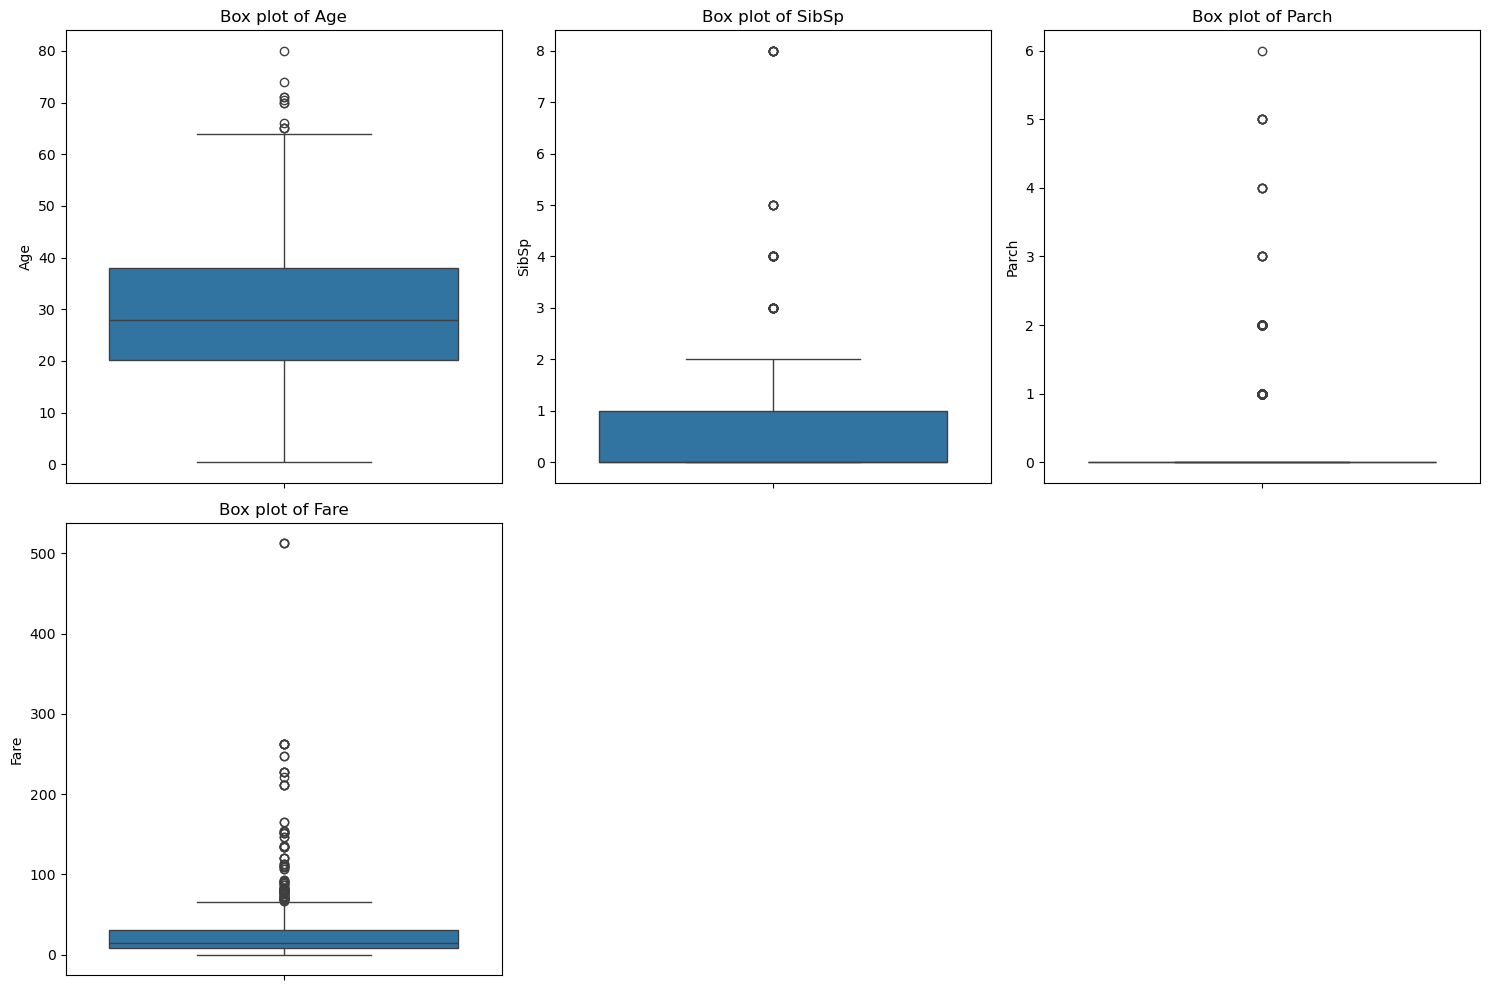
\includegraphics[height=9cm]{analysis_files/analysis_2_0.png}
	\caption{Box plots of the variables Age, SibSp, Parch, and Fare.}
	\label{figure:initial-box-plots}
\end{figure}

The Age and Fare attributes on the other hand are much more interesting. We can see that there are some outliers in the data. Values above the highest whiskers represent the outliers. For Age the ones slightly above 60 are outliers, and for Fare, the ones above around 80 look to be outliers.

We believe that the outliers are still fundamental when it comes to analysis of survivability of a passenger, and Age and Fare prices are believed to be important factors, so we want to keep these. The only outlier we would remove would be the fare price of 512.3292. This results in the box plots of figure \ref{figure:final-box-plots}.

\begin{figure}[h!]
	\centering
	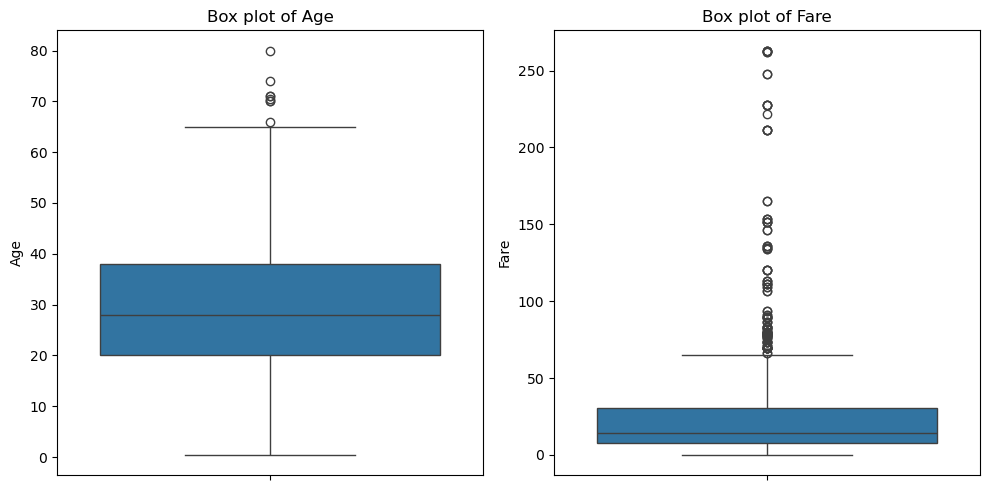
\includegraphics[height=6cm]{analysis_files/analysis_3_0.png}
	\caption{Box plots of Age and Fare with Fare outlier removed.}
	\label{figure:final-box-plots}
\end{figure}

\subsection*{Do the attributes appear to be normally distributed?}

In order to determine that, we first need to observe our dataset and check if the observations in each attribute are continuous. This is because the normal distribution is continuous. From our analysis in question 2, we see that age and fare are two continuous attributes. One simple way to acknowledge if the data is normally distributed is to plot a histogram as is done on figure \ref{figure:histogram}.

\begin{figure}[h!]
	\centering]
	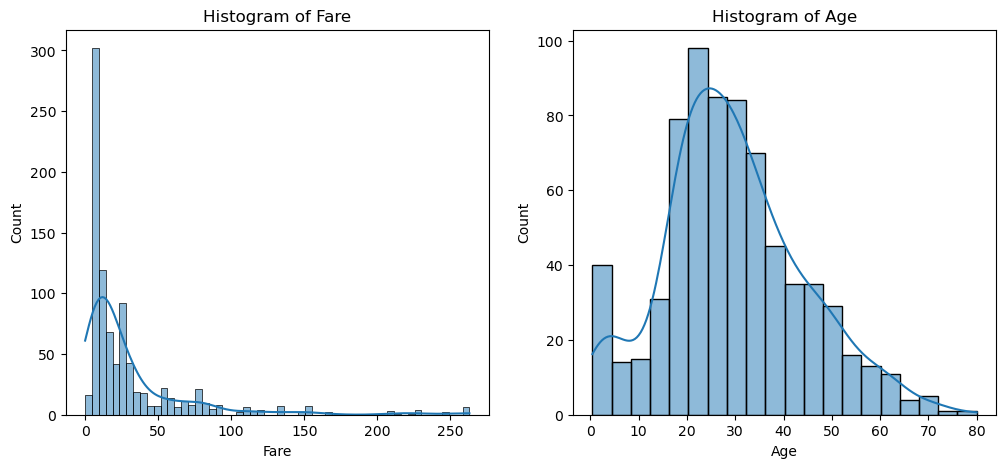
\includegraphics[height=7cm]{analysis_files/analysis_4_1.png}
	\caption{Histogram of Age and Fare}
	\label{figure:histogram}
\end{figure}
    
We can see that the result above shows that the data is not very normally distributed. Age is slightly bell shaped, but it skews slightly to the right whilst the fare distribution is heavily skewed to the right. This is due to the numerous outliers present in the attributes. If we want to normally distribute them more, we would have to log transform to reduce skewness.

\subsection*{Are the variables correlated?}

We can use a correlation matrix to determine if the variables are correlated, but before that, we need to encode categorical variables as numerical ones. There are several categorical variables, but we believe sex and pClass to be the most significant in determining survivability of a passenger. We compute the correlation matrix as follows:

\begin{tcolorbox}[breakable, size=fbox, boxrule=1pt, pad at break*=1mm,colback=cellbackground, colframe=cellborder]
\begin{Verbatim}[commandchars=\\\{\}]
\PY{c+c1}{\PYZsh{} Make another copy of the dataframe where df contains the entire dataset}
\PY{n}{cor\PYZus{}df} \PY{o}{=} \PY{n}{df}
\PY{c+c1}{\PYZsh{} Code below to encode sex whilst pClass is already numerical}
\PY{n}{label\PYZus{}encoder} \PY{o}{=} \PY{n}{LabelEncoder}\PY{p}{(}\PY{p}{)}
\PY{n}{cor\PYZus{}df}\PY{o}{.}\PY{n}{loc}\PY{p}{[}\PY{p}{:}\PY{p}{,}\PY{l+s+s1}{\PYZsq{}}\PY{l+s+s1}{Sex}\PY{l+s+s1}{\PYZsq{}}\PY{p}{]} \PY{o}{=} \PY{n}{label\PYZus{}encoder}\PY{o}{.}\PY{n}{fit\PYZus{}transform}\PY{p}{(}\PY{n}{df}\PY{p}{[}\PY{l+s+s1}{\PYZsq{}}\PY{l+s+s1}{Sex}\PY{l+s+s1}{\PYZsq{}}\PY{p}{]}\PY{p}{)}
\PY{c+c1}{\PYZsh{} Drop columns that are not of significance}
\PY{n}{cor\PYZus{}df} \PY{o}{=} \PY{n}{df}\PY{o}{.}\PY{n}{drop}\PY{p}{(}\PY{n}{columns}\PY{o}{=}\PY{p}{[}\PY{l+s+s1}{\PYZsq{}}\PY{l+s+s1}{PassengerId}\PY{l+s+s1}{\PYZsq{}}\PY{p}{,}\PY{l+s+s1}{\PYZsq{}}\PY{l+s+s1}{Name}\PY{l+s+s1}{\PYZsq{}}\PY{p}{,} \PY{l+s+s1}{\PYZsq{}}\PY{l+s+s1}{Ticket}\PY{l+s+s1}{\PYZsq{}}\PY{p}{,} \PY{l+s+s1}{\PYZsq{}}\PY{l+s+s1}{Cabin}\PY{l+s+s1}{\PYZsq{}}\PY{p}{,}\PY{l+s+s1}{\PYZsq{}}\PY{l+s+s1}{Embarked}\PY{l+s+s1}{\PYZsq{}}\PY{p}{]}\PY{p}{)}
\PY{c+c1}{\PYZsh{} Compute the correlation matrix}
\PY{n}{correlation\PYZus{}matrix} \PY{o}{=} \PY{n}{cor\PYZus{}df}\PY{o}{.}\PY{n}{corr}\PY{p}{(}\PY{p}{)}
\PY{c+c1}{\PYZsh{} Display the correlation matrix}
\PY{n+nb}{print}\PY{p}{(}\PY{n}{correlation\PYZus{}matrix}\PY{p}{)}
\end{Verbatim}
\end{tcolorbox}
\begin{Verbatim}[commandchars=\\\{\}]
          Survived    Pclass       Sex       Age     SibSp     Parch      Fare
Survived  1.000000 -0.334068 -0.545899 -0.079472 -0.033395  0.082157  0.261742
Pclass   -0.334068  1.000000  0.132881 -0.368625  0.080937  0.018212 -0.604960
Sex      -0.545899  0.132881  1.000000  0.093296 -0.114799 -0.247003 -0.222361
Age      -0.079472 -0.368625  0.093296  1.000000 -0.307639 -0.189194  0.100396
SibSp    -0.033395  0.080937 -0.114799 -0.307639  1.000000  0.415141  0.211816
Parch     0.082157  0.018212 -0.247003 -0.189194  0.415141  1.000000  0.263910
Fare      0.261742 -0.604960 -0.222361  0.100396  0.211816  0.263910  1.000000
\end{Verbatim}

Above we can see the correlation matrix of the various attributes together. We can see that when it comes to sex and survived, there is a moderate negative correlation of -0.54. This suggests that passengers being male (encoded as 1) are less likely to survive. There is also a negative correlation of class and survival, which suggests that passengers in higher classes are more likely to survive. Finally the fare has a relatively moderate positive correlation with survival, which suggests that
passengers who paid more for their fare are more likely to survive. 

When looking away from target variables, we can also see some other correlations passenger class and age, where there's a moderate correlation indicating that higher class has a moderate relationship with increased age. We also see a moderate to strong correlation between the class and the fare indicating that the higher the passenger class of the ticket, the higher the fare price. Other notable and fairly obvious correlations are the instances of siblings and the instances of parents, which have a moderate positive correlation.

\subsection*{Does the primary machine learning modeling aim appear to be feasible based on your visualizations?}

This dataset is primarily a classification problem, where we are trying to predict whether a passenger survived or not. Here the target variable is survived which has a binary outcome, making it suitable for classification problems.

Based on the correlation matrix results, we can see that there are some attributes that are correlated with the target variable
and most are explained in the first paragraph in this cell. Through visualization, we can see that the age and fares are relatively
normally distributed but skewed, especially fares, which could affect the model's performance, which might necessitate
a transformation such as log transformation to reduce skewness.

Classification is the most feasible given the correlation matrix and the visualizations we have done so far, which could include models such as logistic regression and decision trees.

Linear regression could be used to explore the relationship between age and fare, although given the skewness and the weak positive correlation between the two, it might require some additional data manipulation to improve the model's performance.

\subsection*{The principal component analysis}

First thing we need to do is to clean the data to prepare it for PCA. Recall that, PCA works on numerical data. We therefore drop the attributes Name, Ticket, Cabin, and PassengerId as these are qualitative. We further convert the categorical variables Sex and Embarked into indicator variables. The remaining attributes are of interest when it comes to the target variable survivability. Following our conversions, no non-numerical data remains.

One last thing before we apply PCA, we need to standardize the data. This is because PCA is sensitive to the scale of the data. One reason is that if we compare age to fare, age can vary from 0 to 100, whilst fare can vary from 0 to 1000. This means that the variance in the data is dominated by fare. We need to standardize the data so that the variance in the data is not dominated by one attribute. We can do this by subtracting the mean and dividing by the standard deviation of each attribute:

\begin{tcolorbox}[breakable, size=fbox, boxrule=1pt, pad at break*=1mm,colback=cellbackground, colframe=cellborder]
\begin{Verbatim}[commandchars=\\\{\}]
\PY{c+c1}{\PYZsh{} Standardize the data using the StandardScaler import.}
\PY{c+c1}{\PYZsh{} Mathematically this is fairly simple, as it involves Z-scoring the data.}
\PY{n}{scaler} \PY{o}{=} \PY{n}{StandardScaler}\PY{p}{(}\PY{p}{)}
\PY{c+c1}{\PYZsh{} fit calculates the mean and standard deviation of each attribute}
\PY{c+1}{\PYZsh{} and transform applies the Z score formula to each attribute.}
\PY{c+1}{\PYZsh{} df_clean is the cleaned dataset.}
\PY{n}{df\PYZus{}standardized} \PY{o}{=} \PY{n}{scaler}\PY{o}{.}\PY{n}{fit\PYZus{}transform}\PY{p}{(}\PY{n}{df\PYZus{}clean}\PY{p}{)}
\end{Verbatim}
\end{tcolorbox}

All the standardized values show how many standard deviations away from the mean the data is. There is one value that is 4.94 standard deviations away from the mean. Finally, we perform PCA using the singular value decomposition:

\begin{tcolorbox}[breakable, size=fbox, boxrule=1pt, pad at break*=1mm,colback=cellbackground, colframe=cellborder]
\begin{Verbatim}[commandchars=\\\{\}]
\PY{n}{U}\PY{p}{,} \PY{n}{S}\PY{p}{,} \PY{n}{Vt} \PY{o}{=} \PY{n}{svd}\PY{p}{(}\PY{n}{df\PYZus{}standardized}\PY{p}{,} \PY{n}{full\PYZus{}matrices}\PY{o}{=}\PY{k+kc}{False}\PY{p}{)}
\PY{c+c1}{\PYZsh{} Compute variance explained by principal components:}
\PY{n}{rho} \PY{o}{=} \PY{p}{(}\PY{n}{S} \PY{o}{*} \PY{n}{S}\PY{p}{)} \PY{o}{/} \PY{p}{(}\PY{n}{S} \PY{o}{*} \PY{n}{S}\PY{p}{)}\PY{o}{.}\PY{n}{sum}\PY{p}{(}\PY{p}{)}
\end{Verbatim}
\end{tcolorbox}

We define a threshold of 90\% of the variance explained to see how many principal components are needed to explain most of the variance. We plot the variance explained to see how many principal components are needed to surpass this threshold. The plot is seen in figure \ref{figure:variance-explained}.

\begin{figure}[h!]
	\centering
	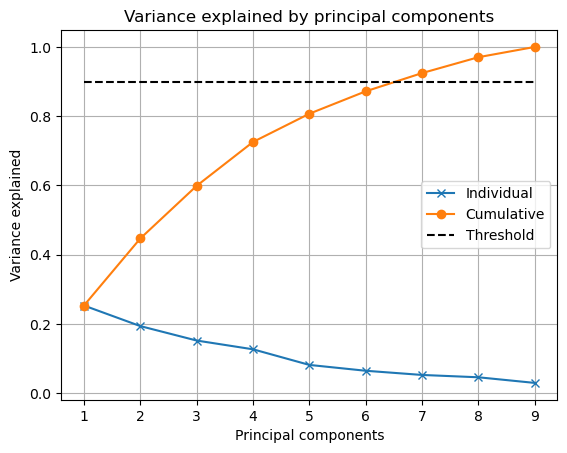
\includegraphics[height=7cm]{analysis_files/analysis_10_0.png}
	\caption{Plot of variance explained by against number of principal components with threshold of 90\%.}
	\label{figure:variance-explained}
\end{figure}

How can we interpret this result? It is obvious from the graph above that we need at least 7 principal components to explain at least 90\% of the variance, which is 2 less dimensions than the cleaned dataset and 6 less dimensions than the original dataset. This is a reduction in dimensionality whilst still being able to explain most of the spread of the original data.

Unfortunately we can only visualize up to 3D data, which in this dataset only amounts to 60\% of the variance explained. This is the tradeoff of PCA, we lose some information but we gain interpretability and computational efficiency.

We will now attempt to interpret the 7 principal components needed to explain 90\% of the variance. This is seen in figure \ref{figure:principal-components}.
    
\begin{figure}[h!]
	\centering
	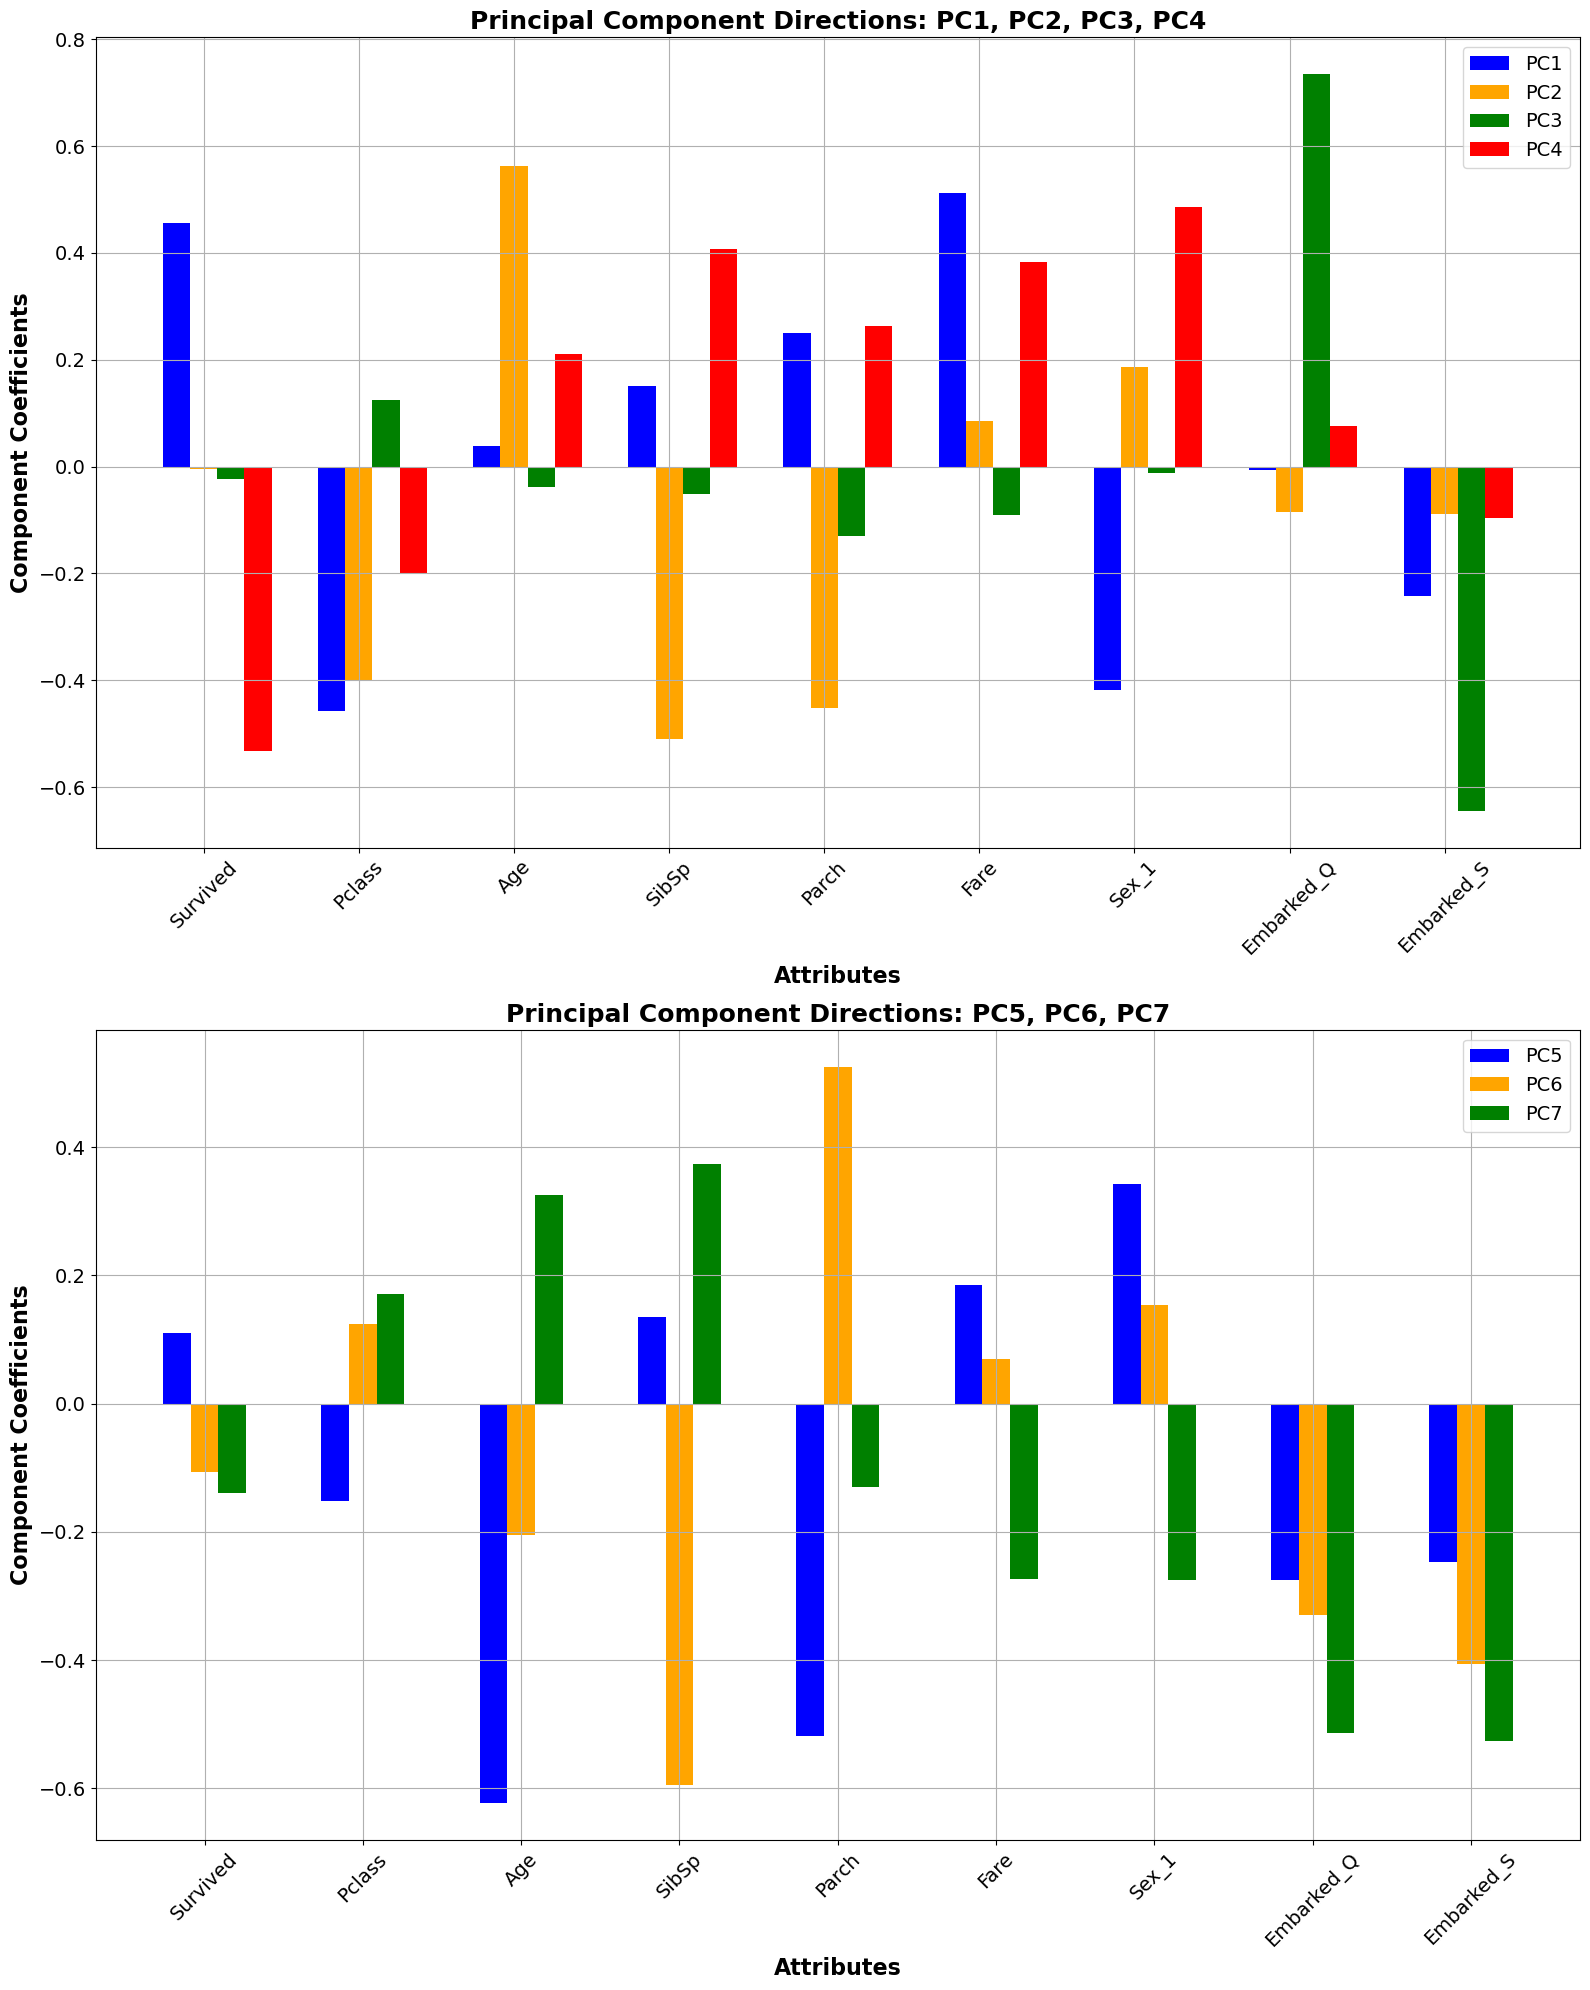
\includegraphics[height=12cm]{analysis_files/analysis_11_1.png}
	\caption{The principal components' values on each attribute.}
	\label{figure:principal-components}
\end{figure}
    
How can we interpret this? Each principle direction is an eigenvector orthonormal to each other where the direction yields the maximized variance of the projected datapoints. The first principle component always yields the highest proportion of the variance. This then tapers as we move onto the next few principle components.

The bars represent the contributions of each feature to the principle component, where the sign either positive or negative and magnitude of these coefficients indicate the direction and strength of each feature's contribution. A positive bar means that the feature contributes positively to the component and vice versa. Magnitude shows the strength of each contribution.

We interpret each of the principal components to capture the following patterns:

\begin{itemize}
	\item Principal component 1: Attributes like ``Survived'', ``Sex\_1'', ``Fare'' and ``pClass'' have relatively high positive coefficients, suggesting they are key factors driving the variance captured by principal component 1. These attributes seem to explain variances concerning socioeconomic status, with survivability being driven by higher class, higher fare prices and not being male.

	\item Principal component 2: The main attribute with the highest magnitude seems to be the positive age. It looks like higher age is associated with higher pClass, not travelling with children, siblings as well as being male and slightly increased fare prices.

	\item Principal component 3: Seems to capture where a person is embarked and it seems like the underlying pattern is that if a person embarked from Q, they certaintly didn't from S.

	\item Principal component 4: Seems to revolve around not surviving the journey and the other bar charts are relatively moderate indicating that if a person was a middleclass male, there seems to be a downward forcing survivability rate.

	\item Principal component 5: Here the underlying pattern seems to be that if a person is young, there seems to be an inverse relationship with number of parents children aboard.

	\item Principal component 6: Looks like this principle component captures the relationship mostly between instances of parents / children aboard and number of siblings aboard, which makes sense as parents with children onboard would often have several children with them.

	\item Principal component 7: Difficult to interpret, maybe a pattern of how a person embarked?
\end{itemize}

\begin{figure}[h!] 
	\centering
	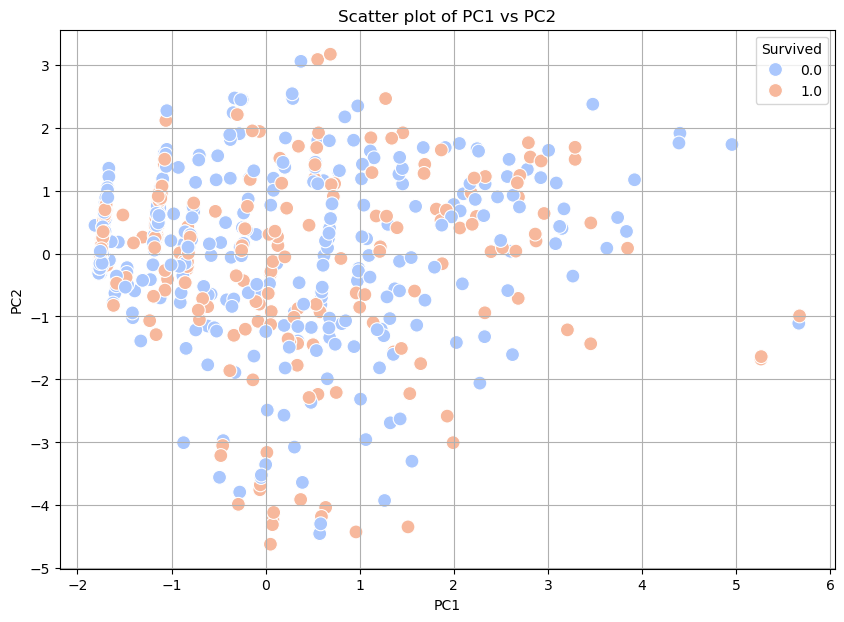
\includegraphics[height=8cm]{analysis_files/analysis_13_2.png}
	\caption{The data projected onto the first two principal components.}
	\label{figure:two-components}
\end{figure}

Now we describe the data projected onto the considered principal components. The 2-dimensional graph seen in figure \ref{figure:two-components} do not separate the two binary outcomes into clear clusters, suggesting that the first two principle components do not capture the variance too well. This makes sense given that the first two principle components only explains a little under half of the variance whilst the optimal solution is to get them to explain at least 90\%. This proved to be only doable with 7 principle components. Maybe projecting to 3 dimensions would ease this.

\begin{figure}[h!]
	\centering
	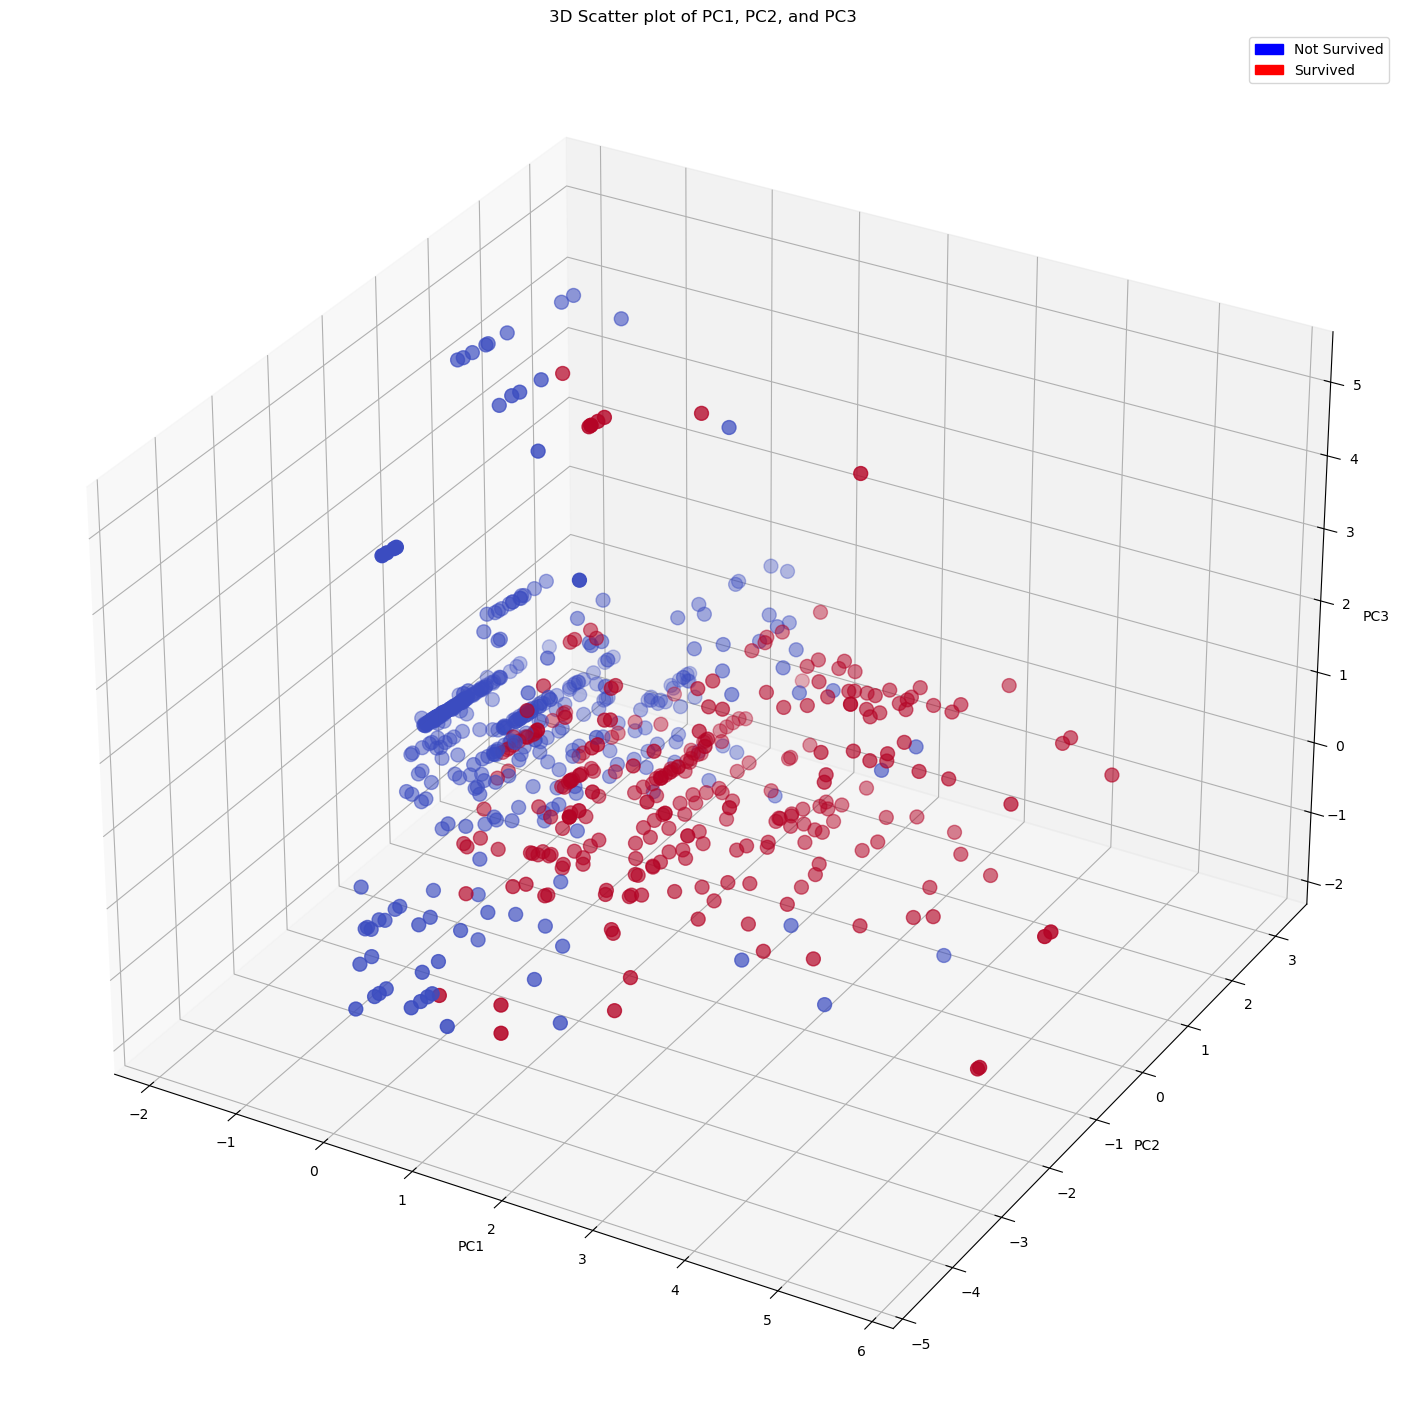
\includegraphics[height=11cm]{analysis_files/analysis_15_0.png}
	\caption{The data projected onto the first three principal components.}
	\label{figure:three-components}
\end{figure}
    
The 3-dimensional graph is seen in figure \ref{figure:three-components}. We get a slightly clearer view here although the first 3 components seem to only capture around 60\% of the variance. Based on what we can observe here, we do see some semblance of two clusters being formed. Based on this static 3D plot, it looks like we can see a cluster for individuals not surviving being formed by low values of principal component 1, relatively high values of principal component 2, and non-positive values of principal component 3.

With negative principal component 1 values, we previously interpreted this as an individual having relatively low socio-economic status, which makes sense given that they were often farther down the ship. We also see that the cluster along principal component 2 seems to be based on being slightly older being a cluster of fatalities there too, which seems to make sense given that younger people, especially children would survive more.

Lastly, principal component 3 is much harder to interpret as it seems to show the relationship based on the embarking of a passenger. The effect of this is unclear.

\section*{Task 4}

In the preceding three task, we have explored the Titanic dataset to assess its quality and suitability for classification and regression tasks. The key interest in the dataset is the possibility of finding patterns in the demographic factors of the passengers that could explain their survival rate. This is a noteworthy problem, as the Titanic carried insufficient lifeboats to save all of its passengers. It is therefore insightful to determine whether the crisis adversely affected certain demographic groups or if survival was arbitrary.

This is by no means a novel analysis. Many previous analyses exist that also deal with the problem of detecting any pattern between the other variables and survivorship. The chief challenge that all prior analyses have faced is the quality of the data. Some variables have missing data. Also, survivorship is not a balanced variable. This results in some data wrangling challenges. However, since most of the variables are typical demographic variables, it should be possible to treat them all using standard techniques, e.g. imputation for missing values, and still obtain decent results.

Our principal component analysis reveals that a significant number of principal components is needed to explain most of the variance in the dataset. This, again, convolutes any potential classification or regression analysis, as many of the datasets dimensions will need to be accounted for. And even with the dimensions accounted for, any clear pattern may not be guaranteed.

However, none of these challenges foreclose statistical analysis. Most datasets are somewhat messy and need cleaning. The Titanic dataset is no different. Our principal component analysis demonstrates that it is possible to make sense of the dimensions captured in the dataset. Prior analyses also demonstrate the feasibility of working with the dataset. We therefore judge that we will be able to complete our classification and regression analyses of the data.

\section*{Exam Problems}

\subsection*{Question 1}

The only correct statement is C. The justification is:

\begin{itemize}
	\item The variable \(x_1\) represents the time of day in blocks of 30 minutes that partition a day into a finite number of intervals. The variable is therefore discrete. Since the intervals can be ordered, the variable is ordinal.

	\item The attribute \(x_6\) is a ratio variable. The number of broken traffic lights is clearly a numeric variable. The cannonical zero of the variable is zero broken traffic lights.

	\item The attribute \(x_7\) is a ratio variable for much the same reasons as for \(x_6\).

	\item The congestion level is ordinal as it is a discrete variable that can be ordered.
\end{itemize}

The statements A, B, and D are all incorrect as they mistake \(x_1\) for something other than an ordinal variable.

\subsection*{Question 2}

\begin{enumerate}[label=\Alph*.]
	\item This statement is correct since \(|26 - 19| = 7\) and that is the maximal difference among the respective coordinates of the two vectors.

	\item The metric is
	\[
		d_3(x_{14}, x_{18}) = \sqrt[3]{|26 - 19|^3 + |2 - 0|^3} \approx 7.05.
	\]
	Thus, the statement is incorrect.

	\item The metric is
	\[
		d_1(x_{14}, x_{18}) = |26 - 19| + |2 - 0| = 9.
	\]
	Thus, the statement is incorrect.

	\item The metric is
	\[
		d_4(x_{14}, x_{18}) = \sqrt[4]{|26 - 19|^4 + |2 - 0|^4} \approx 7.01.
	\]
	Thus, the statement is incorrect.

\end{enumerate}

\subsection*{Question 3}

\begin{enumerate}[label=\Alph*.]
	\item The explained variance is
	\[
		\frac{13.9^2 + 12.47^2 + 11.48^2 + 10.03^2}{13.9^2 + 12.47^2 + 11.48^2 + 10.03^2 + 9.45^2} \approx 0.87.
	\]
	The statement is therefore correct.

	\item The explained variance is
	\[
		\frac{11.48^2 + 10.03^2 + 9.45^2}{13.9^2 + 12.47^2 + 11.48^2 + 10.03^2 + 9.45^2} \approx 0.48.
	\]
	Thus, the statement is incorrect.

	\item The explained variance is
	\[
		\frac{13.9^2 + 12.47^2}{13.9^2 + 12.47^2 + 11.48^2 + 10.03^2 + 9.45^2} \approx 0.52.
	\]
	Thus, the statement is incorrect.

	\item The explained variance is
	\[
		\frac{13.9^2 + 12.47^2 + 11.48^2}{13.9^2 + 12.47^2 + 11.48^2 + 10.03^2 + 9.45^2} \approx 0.72.
	\]
	Thus, the statement is incorrect.

\end{enumerate}

\subsection*{Question 4}

\begin{enumerate}[label=\Alph*.]
	\item Such an observation will typically have a negative value as the high values of the third and fourth coordinates will make the negative coordinates of the principal component dominate. The statement is false.

	\item For much the same reasons as in A, such an observation will typically have a negative value. This statement is false.

	\item For such an observation, the positive value of the second coordinate of the principal component will dominate the sum in the dot product. The value will therefore typically be positive. The statement is false.

	\item The only negative coordinate of the principal component is the first one. As the observation has a low value in this position, and high values everywhere else, the dot product will typically be positive. The statement is correct.
	\end{enumerate}

\subsection*{Question 5}

We are given the following data:
\[
	n = 20000, M_{11} = 2, M_{01} = 5, M_{10} = 6.
\]
The Jaccard similarity of the documents is
\[
	\frac{M_{11}}{M_{11} + M_{01} + M_{10}} \approx 0.1538.
\]
The correct answer is A.

\subsection*{Question 6}

The probability \(p(\hat{x}_2 = 0 \, | \, y = 2)\) can be found by marginalizing on \(\hat{x}_7\). This results in the probability
\[
	p(\hat{x}_2 = 0 \, | \, y = 2) = p(\hat{x}_2 = 0, \hat{x}_7 = 0 \, | \, y = 2)
	+ p(\hat{x}_2 = 0, \hat{x}_7 = 1 \, | \, y = 2) = 0.81 + 0.03 = 0.84.
\]
The correct answer is B.

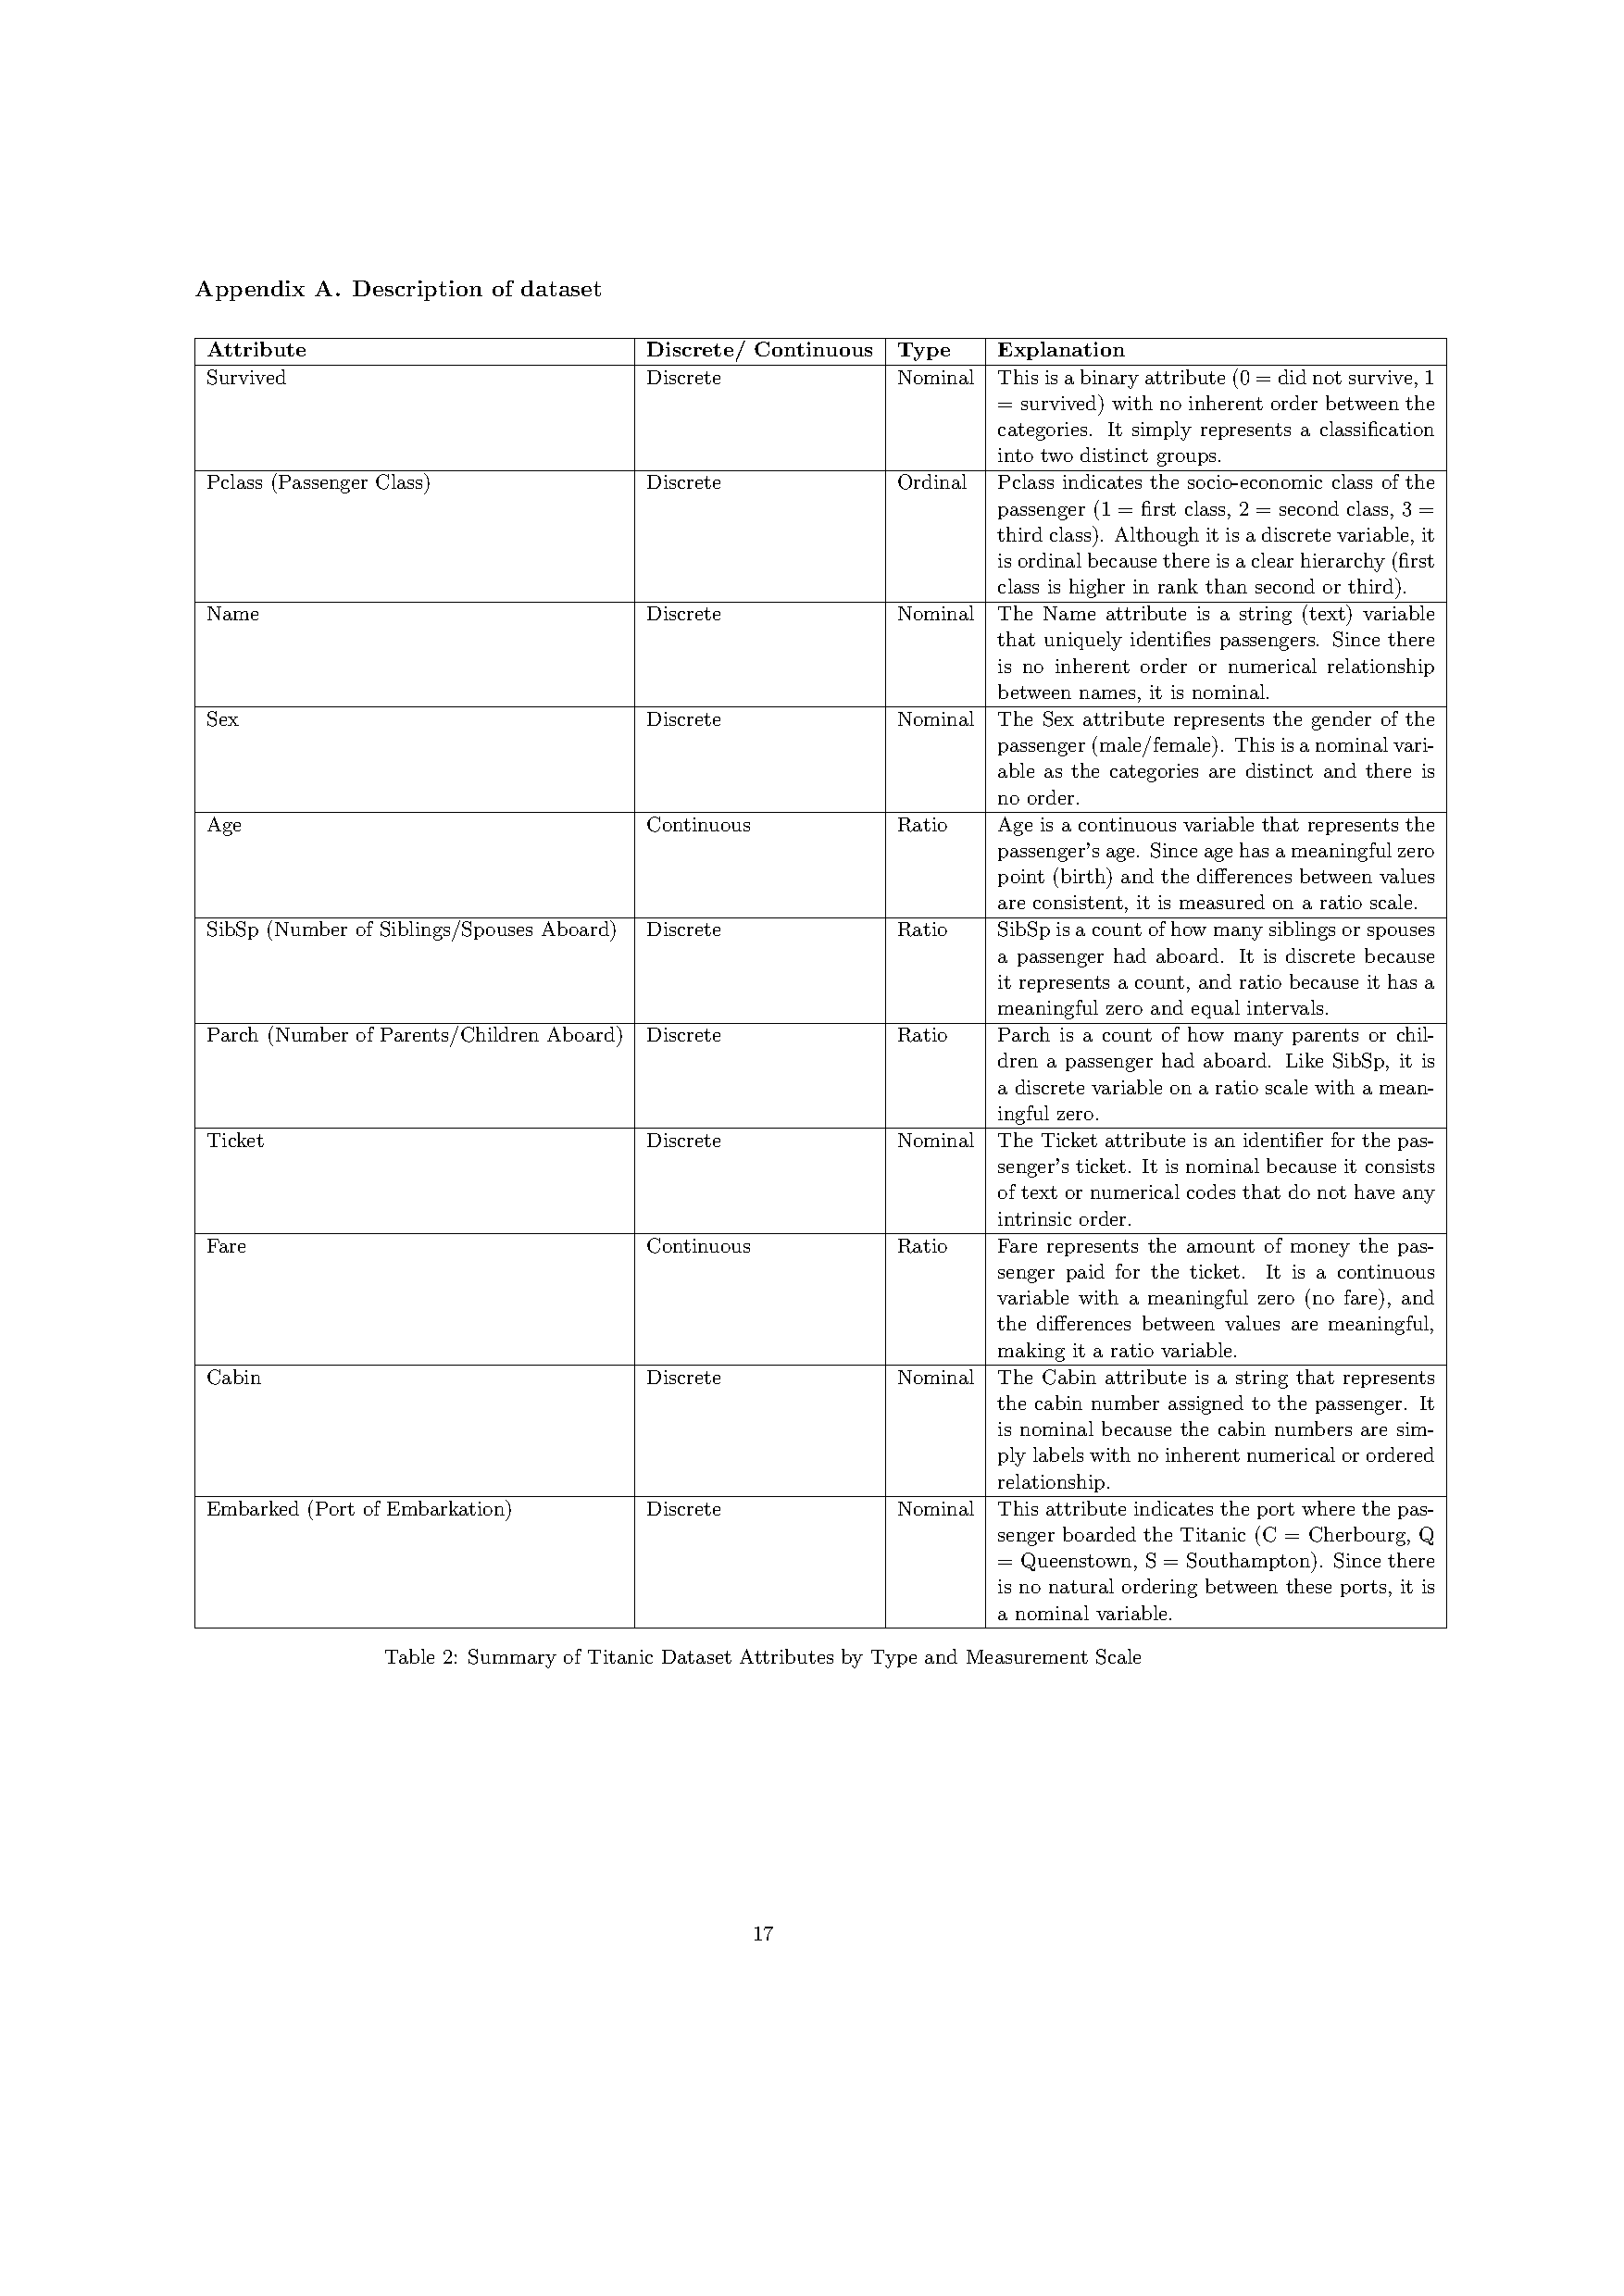
\includepdf[
	pages=1,%
	addtolist={%
		1,%
		table,%
		{Description of the dataset},%
		table:description%
	}%
]{table}

\bibliography{references}

\end{document}
